\chapter{Concluding remarks}\label{ch:conclusion}

\setlength{\epigraphwidth}{0.49\textwidth}%0.57
    \setlength{\epigraphrule}{0pt}%0.1
    \epigraphhead[5]{%
    \epigraph{\emph{Has been done. Can be done. Must be done\ldots}}%
    {Fandarel \mycite{McCaffrey}}
}


With the recent profusion of expression atlases,
notably for human,
it has become increasingly imperative to examine
the soundness of their extensive use in other (unrelated) studies.
Especially given the number of articles integrating
these atlases' data as-is is steadily and rapidly growing
(more than 2,800 citations on the 15 September 2019 for five studies).

At the time I started my doctorate,
no assessment on the robustness of expression or
comparison between independent \Rnaseq\ datasets was published yet.
Thus,
my primary aim was to integrate and compare independent transcriptomic data
as they were the only available human tissue data.
However, the release of two substantial proteomic datasets in the meantime
broadened my study's scope
to the integration of transcriptomic with proteomic data too.

In \Cref{ch:background},
I review all the biology, chemistry and bioinformatic aspects and challenges
involved in expression studies based on the high-throughput technologies
of \Rnaseq\ (for \mRNAs) and \ms{} (for proteins).

Then in \Cref{ch:datasets},
I present the five transcriptomic studies and three proteomics studies
that I have considered for further analyses.
I also detail the pipelines with which I have processed them.
Since the amount of each dataset files is extremely important,
automation is paramount to ensure consistency and minimise errors.\mybr\

\Cref{ch:expression} details various data quality controls
and statistical approaches.
I also discuss possible biases and
how the contextual scope of which tissues and genes are considered for analyses
can influence their results.
To minimise errors due to context issues,
I limit most of my further investigations to
a common subset of tissues and expressed genes.
%I also aggregate in each dataset
%the expression of all samples of the same tissue in
%one \trep\ (tissue reference expression profile).
%Finally,
I also remove mitochondria genes from most of the analyses.
Indeed, current normalisation methods are inadequate to quantify them.

In \Cref{ch:Transcriptomics},
I integrate the five independent transcriptomic datasets.
There is an evident prevalence of the biological signal over technical noise.
All datasets have a higher interstudy correlation for the same tissues
than any intrastudy correlation for different tissues.
More recent the studies are, stronger this trend is.
Besides,
the most variable genes and Tissue-Specific (\gls{TS}) genes are contributing
more to the high correlations than the highest expressed ones.
However, the inclusion of external resources requires caution,
especially when the resources are outdated, such as \gls{TIGER}~\mycite{tiger}.

The integration has revealed that
direct comparisons of the raw data may be impossible yet,
but genes present identical overall profiles across the studies.
This similarity prompted the creation of the heatmap visualising expression data
(and its associated widget) for baseline expression data in
\hFoCi{Expression Atlas}{https://www.ebi.ac.uk/gxa/home}{EBIgxa}.
Finally, I provide a core set of genes that are expressed consistently
(ubiquitously or \gls{TS}) across all the studies.

The comparison of three available proteomic datasets
in \Cref{ch:proteomics} highlights
the fragmentation and the disparity of the high-throughput \ms{}-based proteomics.
\ms\ detection variability induces considerable technological noise,
which explains
why intrastudy correlations between different tissues are
higher than the interstudy correlation for the same tissues.
I provide curated sets of ubiquitously and \gls{TS} proteins.
Finally, I present a new quantification method (implemented by \james) that
I have devised by drawing on \Rnaseq\ methods.
This \PPKM\ method allows us to quantify more proteins
by also accounting for \emph{degenerated} peptides.
These latter are distributed according to the distribution of \emph{unique} peptides
between the possible parent proteins.

\Cref{ch:Integration} integrates independent proteomic and transcriptomic data.
I have found similar correlation levels
(Spearman correlation $0.39 ≤ \rho\ ≤ 0.62$)
than the ones typically observed in
the literature for same-sourced proteome and transcriptome.
The \PPKM\ quantification improves the Pearson correlation
and gives similar ranges to Spearman ($0.38 ≤ r ≤ 0.61$).
Two tissues exhibit distinct characteristics across the various analyses
(and literature): \Testis\ and \Liver.
\Testis\ has the most diverse and specific expression
at both transcriptomic and proteomic levels.
On the other hand, \Liver\ has the most robust expression across studies
and the highest correlation between its \mRNAs\ and proteins expression levels.
Overall, the tissues feature mixed correlation levels,
and it is impossible to predict protein expression from \mRNA{}.

However, there are shared coherent gene signatures
between the proteome and transcriptome
that are even detectable through indirect analyses for a few.
Besides, once again,
\mRNAs{}' and proteins' tissue specificity is contributing
more to the tissue correlation than their expression levels.
In addition to the significant overlaps of \gls{TS} proteins
with the most \gls{TS} \mRNAs,
pairs including a \gls{TS} protein have,
in most cases,
a correlation among the highest observed for genes across tissues.
Finally, \gls{go} analyses show that pairs with a \gls{TS} protein
are enriched for specific signalling
(including its detection, response pathway and regulation).
The highest correlated genes (except the ones with a \gls{TS} protein) are
enriched for catabolic processes.
Lastly, the most anticorrelated pairs show enrichment
for ribosome complexes and \glspl{ncRNA} regulation.
I provide the complete set of \mRNA/protein pairs with their correlation
across the common set of tissues.
I also supply the list of overlapping \gls{TS} proteins and \mRNAs{}.

I also provide all the necessary code to replicate all the above results (and more)
as \href{https://github.com/barzine/BaselineAtlas/tree/thesis.}{supplementary
material}\footnote{\Href{https://github.com/barzine/BaselineAtlas/tree/thesis}}.


Throughout this thesis' analyses,
I had to overcome many practical challenges.
While most of the difficulties encountered ordinarily pertain to Big data projects,
one unexpected challenge was
the current global complexity state of the proteomic world.
Physicochemical properties of the proteins make them
intrinsically complex to study,
as shown in \Cref{sec:exploreProtMS}.
However, the overall disparity
when it comes to proteomic studies,
including in terms of learning about general practices and concepts,
was surprising for me.

Big data is often characterised through, what was first defined by
\href{https://www.ibm.com}{IBM}\footnote{\Href{https://www.ibm.com}},
the \emph{4 V's}: volume, variety, veracity and velocity.
Each of them can entail issues at different project levels.

The volume of files (see \Cref{tab:Lib5DF})
to handle and process just for the transcriptomics
is overwhelming and requires properly dimensioned infrastructure
like in the \gls{EBI}.
It is in practice impossible to reproduce the complete work underlying
this thesis in a personal computer within a reasonable time.
Although (commercial) solutions are in use more and more every day
for academic projects,
dedicated storage and high computing facilities ease the analyses considerably
and allow more in-depth testing.
Even if best practices are more and more defined for transcriptomics,
there are still many factors that can be improved and tuned.
Hence, besides the raw data,
storage capacity is also required for the intermediate and final ones.
While in the \gls{EBI} the storage space was large enough,
I overlooked the organisation of the different studies' files,
and I had to change it several times.

The variety of the input data is kept to a minimum for the expression value
as it was retrieved from public or academic repositories
that follow community guidelines\footnote{%
\href{https://www.ebi.ac.uk/ena}{ENA} for the sequencing data and
\href{http://www.proteomexchange.org/}{ProteomeXchange} for \ms/\ms/ proteomics.
}.
Issues still ensue from the matchmaking
between the samples or tissues across the studies.
For many tissues, I chose to mix several \enquote{body parts}
(from the same tissue though) in \gtex\
to match them to the other studies' tissues.
Perhaps, in some case, one \enquote{body part} is perfectly matched
to the samples from another study
where the authors have only reported the tissue instead.

Another source of variety that I have limited in the above work
is the diverse annotation versions.
Even though we mapped both proteomics and transcriptomics
to the same genome and annotation versions,
there are discrepancies in how transcriptomics and proteomics
are defined and mapped to the genome.
A possible improvement of the present work will be to use
the chromosome coordinates to which \mRNAs\ and proteins map
instead of using the gene identifier (\gls{Ensembl} ID).\mybr\

In addition, with all possible tunable parameters for the raw data processing,
the generated data to integrate can vary quickly.
While I lack providing an extensive view of
the impact of the different settings combinations,
my study has shown that the overall trend of the results remains the same.
Moreover, as the number of datasets I include in my analyses has grown,
the results got stabler and stabler.
Many of them have also been confirmed by the literature,
adding credibility to the findings trends
and which is reassuring when
considering the recent discussions on reproducibility crisis~\mycite{%
Morrison2014-hy,Glenn_Begley2015-fz,Goodman2016-ri,Fatovich2017-lo,
Coiera2018-vf,Lindner2018-qy}.
However, caution is still needed when considering individual genes.\mybr\

Finally, the velocity of new data availability
and its required preparation time
before possible inclusion in my on-going analyses
made the prospect unappealing and impracticable.
Unfortunately, although new \gtex\ samples or other tissues studies
(\eg\ Oncobox Atlas of Normal Tissue Expression (ANTE)~\mycite{Suntsova2019-it})
kept being released,
I have stopped comprising them in my study.
Likewise, I ceased updating the genome and annotation
and settled for \hg{38.p1} and \ens{76}.

In order to minimise errors,
assure consistency and ease future reiterations of these analyses
(either for possible extension or just for repeatability sake),
I provide script files that can reproduce the whole study and its results.
I have also automated and structured the analyses trough modular functions
as much as possible.
It is important to avoid undocumented manual changes,
so even name changes and sample pairings are done through scripts.

I chose to develop the analyses with open source software
around the programming language \WebFoCi{\textsf{R}}{https://cran.r-project.org/}{coreR}.
This language provides statistical and visualisation functions
and is easily expanded through packages developed by the community.
A few disadvantages exist with such a framework:
often, while installing or updating a package to gain new features,
other packages will potentially break and require updates.
In many occasions, I will ultimately have to rewrite part of my code.
Furthermore, installing new dependencies for these packages can be challenging
on distributed computing facilities compared to one personal computer.
Fortunately, the older the updated package, the less it induces changes.
Besides, for new projects, one can nowadays employ dedicated packages
(\eg\ \softCi{Packrat}{Rpackrat})
to work in isolated environments and
prevent these chains of \enquote{\emph{update, break, debug/recode}},
which are especially frustrating in exploratory phases.
See \Cref{sec:Rpackages} for the complete list of \textsf{R} packages
involved in this work.

Note that as \nuno, who provided me with the quantification of the \gtex\ data,
and \james, who provided me with the proteomics ones,
have also both developed their processing pipelines with open source software,
the entirety of the thesis (subject to access to \gtex\ data)
can be redone easily by anyone.

I am currently compiling the most pertinent analyses
into a set of interactive applications
that can replicate all the results and figures presented in this thesis
without requiring prerequisite programming skills.
\Cref{fig:demoApp} shows the part covering \Cref{ch:expression}.

\begin{figure}[!ht]
    \frame{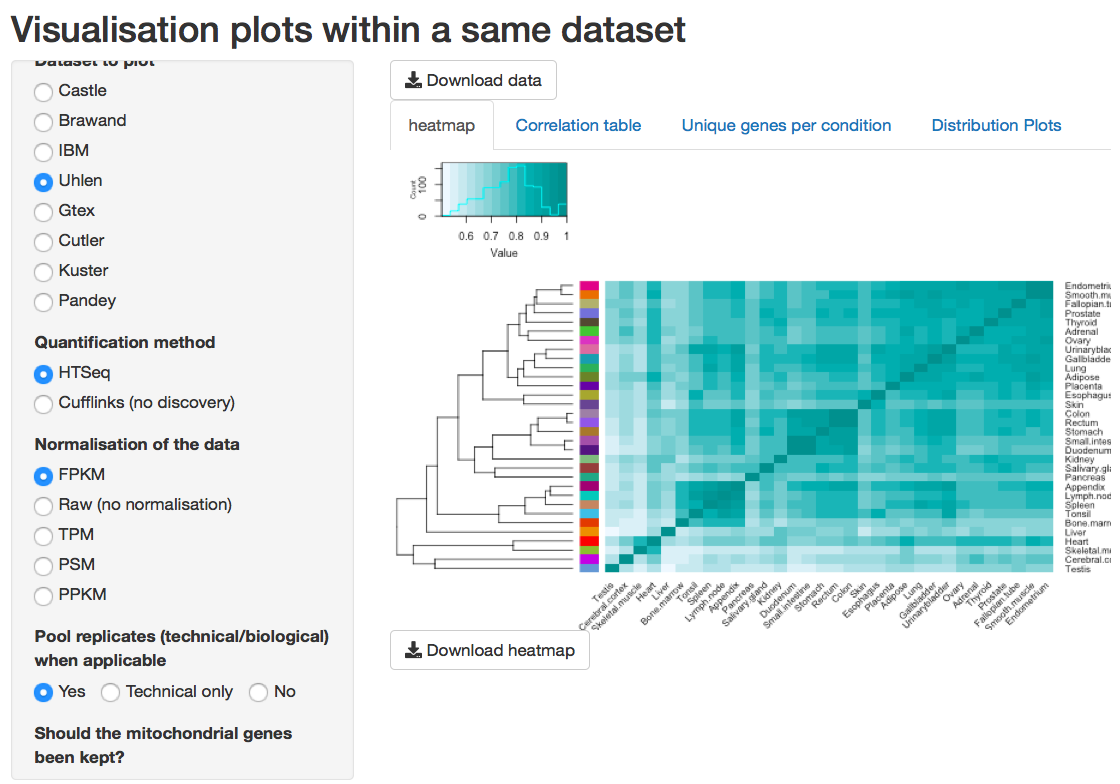
\includegraphics[scale=0.36]{conclusion/demoApp.png}}\centering
    \vspace{-2mm}
    \caption[Application preview]{\label{fig:demoApp}\textbf{Preview of the
    application} developed with \textsf{R}
    and served through a shiny server~\mycite{shinyR}.}
\end{figure}

Many improvements are conceivable:\begin{itemize}
        \item The inclusion of new samples and dataset of transcriptomics
            (preferably with biological replicates),
            \eg\ extend to the last version of \gtex\ and
            the ANTE dataset~\mycite{Suntsova2019-it}.
        \item Add the matching proteomics of \citet{Wang2019-ut}
            to the transcriptomic \uhlen\ data~\mycite{Uhlen2015}
            and then compare the results to the unmatched samples.
        \item Work on new models of annotation or
            build a consensus between the current transcriptomic and proteomic
            annotations.
            At the moment, it is rather difficult to determine for some genes
            (\eg\ \gene{STAU2})
            if the anticorrelation or the lack of correlation observed
            between the expression of its \mRNA\ and protein is due to biology,
            batch effect or the divergence between the transcriptomic and
            proteomic annotations.
        \item Changing the quantification (parameters or methods)
            may also give better results.
\end{itemize}

On this latter point 




%Achievements
% Showed that mitochondrial \mRNAs\ and proteins should be excluded from the bulk
% (even though separate analysis can be considered)
%
% Transcriptomics present similar profiles: tissue across datasets,
% and \mRNAs\ profiles through the tissues across datasets.
% This finding has prompted the EBI heatmap visualisation
%
% New proteomics quantification methods inspired on transcriptomic ones
% can increase the number of quantified proteins
% while seemingly unkooky
%
% First time so many different data have been mapped to the same genome version
% and annotation with identical pipelines.
% Quite in-depth comparison between Uhlen and \gtex.
% Reprocessing of all the untarget non-diseased human proteome
%
% Consolidated gene lists for consistent transcriptomic expression
%                                           (modified Uhlen categories)
%                 and for matched (but independently sourced) \mRNA/protein pairs
%                     for TS, highly correlated and very anticorrelated
%
% Organs show constant catabolic profile (set of genes) that have
% mRNAs/proteins expression consistent through aggregation of individual and 
% across different datasets.
% Particularly, housekeeping and TS genes
%
% Testis most diverse and unique expression
% Liver most robust expression
%

